\documentclass[conference]{IEEEtran}
\IEEEoverridecommandlockouts
% Draft paper dari Tugas Akhir 18222028 — Erwan Poltak Halomoan
% Template: IEEE conference (IEEEtran.cls V1.8b, bundel resmi 17 Okt 2019)
% Direvisi 7 Agustus 2026 agar konsisten dengan buku TA final (TA.pdf, 212 hlm).
% Seluruh angka tertelusur ke results/experiments/analysis/ atau ke tabel buku.
% Keperluan: syarat yudisium. Belum ditujukan ke konferensi tertentu;
% format mengikuti IEEE conference standar dengan anggaran 6 halaman.

\usepackage{cite}
\usepackage{amsmath,amssymb,amsfonts}
\usepackage{graphicx}
\usepackage{textcomp}
\usepackage{xcolor}
\usepackage{booktabs}

\def\BibTeX{{\rm B\kern-.05em{\sc i\kern-.025em b}\kern-.08em T\kern-.1667em\lower.7ex\hbox{E}\kern-.125emX}}

\begin{document}

\title{Development of a BI-Rate Prediction System Based on Explainable Artificial Intelligence (XAI) and a Large Language Model (LLM) Using Macroeconomic Indicators}

\author{\IEEEauthorblockN{Erwan Poltak Halomoan}
\IEEEauthorblockA{\textit{Information System and Technology} \\
\textit{School of Electrical Engineering and Informatics} \\
\textit{Institut Teknologi Bandung} \\
Bandung, Indonesia \\
18222028@mahasiswa.itb.ac.id}
\and
\IEEEauthorblockN{Windy Gambetta}
\IEEEauthorblockA{\textit{School of Electrical Engineering and Informatics} \\
\textit{Institut Teknologi Bandung} \\
Bandung, Indonesia \\
windy@itb.ac.id}
}

\maketitle

\begin{abstract}
The BI-Rate, Bank Indonesia's policy rate, has broad implications for the national economy, yet the process behind its determination is widely perceived as a black box. This paper presents a prediction system integrating three components: a prediction module comparing six econometric and machine learning models (ARIMA, VAR, Random Forest, XGBoost, LSTM, BiLSTM); an Explainable AI layer combining SHAP and LIME; and a narrative layer in which GPT-4o converts XAI output into reports for non-technical stakeholders. Using 251 monthly observations (July 2005--May 2026) of 12 macroeconomic indicators, models were evaluated over a factorial design of 384 preprocessing combinations. On aggregate metrics Random Forest, BiLSTM, and LSTM are best and practically equivalent (RMSE 0.14--0.16, $R^2$ 0.86--0.89), while econometric baselines fail. Because the BI-Rate is highly persistent, change and hold months are assessed separately, and the ranking reverses: on the nine rate-change months BiLSTM and LSTM reach 67\% directional accuracy against 33\% for the aggregate winner Random Forest. Leave-one-out ablation locates that capability in the macroeconomic block rather than in persistence---removing BI-Rate $t-1$ raises Random Forest RMSE from 0.143 to 0.409 yet leaves both recurrent models unchanged, and a lag-only variant is more accurate in aggregate but collapses to 0--22\% directional accuracy on change months. SHAP attributes 75.5\% of Random Forest's contribution to persistence but only 7--10\% for the recurrent models, and LIME's local surrogate fit is poor (median $R^2$ 0.025), confining it to a direction check. A Bank Indonesia monetary economist scored the narratives 3.99 of 5, with hallucination-absence and SHAP-consistency items receiving full marks.
\end{abstract}

\begin{IEEEkeywords}
BI-Rate, interest rate prediction, explainable AI, SHAP, LIME, large language model, monetary policy, time series
\end{IEEEkeywords}

\section{Introduction}
The BI-Rate anchors inflation expectations, exchange-rate stability, and credit conditions in Indonesia. It is set monthly by the Board of Governors of Bank Indonesia, moves gradually in 0.25 percentage-point steps, and, while theoretically grounded in Taylor-rule reasoning \cite{taylor1993}, reflects a far richer set of considerations in practice. Although the underlying macroeconomic data are public, no quantitative account of each indicator's contribution to the decision is available, so the process is widely perceived as a black box.

Machine learning (ML) and deep learning (DL) models capture the nonlinear interactions among macroeconomic indicators better than traditional econometrics \cite{chakraborty2017}, but they are themselves opaque. In public policy settings accuracy alone is insufficient: stakeholders require explanations that can be audited and challenged. Explainable AI (XAI) methods such as SHAP \cite{lundberg2017} and LIME \cite{ribeiro2016} address attribution, yet their raw outputs---plots and matrices of values---remain unfriendly to non-technical decision makers. Research combining ML/DL prediction, XAI attribution, and large language model (LLM) narration for the Indonesian policy rate is still scarce.

This paper develops and evaluates such a pipeline end to end and makes four contributions:
\begin{enumerate}
    \item a reproducible factorial benchmark of 384 preprocessing combinations $\times$ 6 models for BI-Rate prediction, with a locked results registry;
    \item a persistence-aware evaluation protocol that separates rate-change from rate-hold months and, together with leave-one-out ablation, shows both that aggregate accuracy is misleading on this highly persistent series and where the models' remaining usefulness actually resides;
    \item a two-layer transparency stack: exact TreeSHAP attribution with LIME as an independent direction check, narrated by GPT-4o under strict grounding constraints so that every quantitative claim is traceable to a SHAP value; and
    \item an expert validation of the explanation quality by a Bank Indonesia monetary economist using a 96-item Likert instrument.
\end{enumerate}

We report the unfavourable findings openly. Aggregate accuracy on this series is largely inherited from interest-rate smoothing, which the system itself quantifies; a three-feature lag-only variant is more accurate in aggregate than the full configuration; and ten of seventeen features lower the average test error when removed. What survives these checks is a narrower but defensible claim, and it is the claim this paper makes: the models' predictive value is concentrated in the months when the policy rate actually moves, it comes from the macroeconomic block rather than from persistence, and it is accompanied by a transparency layer whose outputs an expert can verify line by line.

\section{Related Work}
Chakraborty and Joseph \cite{chakraborty2017} established that ML models outperform traditional benchmarks in central-banking prediction tasks, while noting that interpretability barriers hinder adoption in policy. Bussmann et al. \cite{bussmann2021} paired XGBoost with SHAP for credit risk management, and \c{C}al{\i}k et al. \cite{calik2025} demonstrated SHAP- and LIME-based transparency for transformer stock-price predictors. On the narrative side, Yu et al. \cite{yu2023} explored LLMs for explainable financial time series. The predictive components used here---random forests \cite{breiman2001}, gradient boosting \cite{chen2016}, recurrent architectures \cite{hochreiter1997,schuster1997}, and Optuna \cite{akiba2019} for hyperparameter search---are established workhorses. To our knowledge, however, no prior work integrates factorial preprocessing benchmarking, exact tree attribution with cross-method validation, and grounded LLM narration for Indonesia's policy rate, nor validates the resulting explanations with a central-bank domain expert.

\section{Data and Methodology}
\subsection{Data}
The dataset comprises 251 monthly observations from July 2005 to May 2026 with 12 domestic and global indicators from official sources (Bank Indonesia, Statistics Indonesia/BPS, FRED, CBOE, Yahoo Finance): inflation, the inflation gap, and GDP growth; M2 and outstanding credit; the USD/IDR rate, the equity index, and foreign reserves; and the Federal Funds Rate, Brent oil, gold, and the VIX. Derived features---three BI-Rate lags, the real interest rate, the output gap, inflation momentum, exchange-rate pressure, the change in the Federal Funds Rate, the Fed cycle, and a policy-stance indicator---are produced by the policy-reaction feature-engineering strategy described below, not taken from source data. Missing values are imputed causally with forward fill---the winning strategy in the factorial search---which uses only past information.

All reported figures come from a single computing environment (macOS, Python 3.10). This matters for XGBoost, which yields a different test RMSE on Windows (0.196) than on macOS (0.221) despite identical data, splits, and seeds; the macOS figure is used throughout for internal consistency. The other five models are portable across the two platforms.

\subsection{Factorial Experimental Design}
Preprocessing choices are treated as experimental factors: 4 imputation methods $\times$ 4 feature-selection strategies $\times$ 3 scalers $\times$ 8 feature-engineering strategies, yielding 384 valid combinations evaluated in a five-phase funnel: (1) screening of all combinations with fast tree models; (2) factor analysis isolating each factor's marginal effect; (3) focused evaluation of the top-10 combinations on all six models; (4) hyperparameter tuning (Optuna TPE \cite{akiba2019}, 20 trials for the tree ensembles and 15 for the recurrent networks); and (5) final comparison. Data are split chronologically 60/20/20 without shuffling to prevent temporal leakage, and scalers are fit on training data only. Five further months (January--May 2026) enter none of the three splits and influence no configuration choice; they are forecast with the final models as an additional check on recent data (Section~\ref{sec:robust}). Canonical results are stored in a locked registry so that pipeline reruns cannot silently overwrite reported numbers.

Factor analysis measured each factor's marginal RMSE range over the screening grid. Feature engineering was the most influential (0.7444, led by a policy-reaction feature block), followed by feature selection (0.6892), imputation (0.4275, causal forward fill winning), and scaling (0.0009, negligible for tree models). Feature selection carries a caveat worth stating explicitly: averaged over the whole grid, mutual-information and all-feature selection outrank the expert-curated ITF set, and the expert set wins only at its own best configuration---which is nonetheless the configuration the three leading models adopt.

\subsection{Models}
Six models from two families are compared: ARIMA and VAR as econometric baselines (orders selected by information criteria); Random Forest \cite{breiman2001} and XGBoost \cite{chen2016} as tree ensembles; and LSTM \cite{hochreiter1997} and BiLSTM \cite{schuster1997} as recurrent networks. The networks predict a residual correction anchored at $y_{t-1}$ (residual anchoring) and are trained as three-seed ensembles (seeds 42/43/44) whose predictions are averaged to damp training stochasticity. Inter-run variability was quantified over ten seeds and all 120 three-seed ensembles they generate: the ensemble RMSE standard deviations are $\pm$0.009 (BiLSTM) and $\pm$0.015 (LSTM). Predictions are snapped to the 0.25 percentage-point policy grid for reporting only; all metrics are computed on raw continuous predictions.

\subsection{Explainability Layer}
Global attribution uses exact TreeSHAP on the Random Forest \cite{lundberg2017}; KernelExplainer covers the recurrent models; local per-month explanations (SHAP waterfalls) are produced for all four ML/DL models in both a correctly predicted and a mispredicted month. LIME \cite{ribeiro2016} serves as an independent cross-check of the local attributions, subject to the surrogate-quality caveat reported in Section~\ref{sec:xai}.

\subsection{Narrative Layer}
GPT-4o receives a JSON payload containing only the SHAP values and observed indicator movements for the month being explained. A strict system prompt forbids introducing facts beyond the payload, requires influence magnitudes as percentages of total absolute contribution, phrases directions as ``pushing up/holding down'' rather than causal claims, and appends a disclaimer that deep interpretation requires an expert. Every number in the narrative is therefore manually verifiable against the SHAP table.

\subsection{Evaluation Protocol}
Accuracy is reported as RMSE, MAPE, and $R^2$. Because the BI-Rate is highly persistent, we additionally split the 36-month test window into 9 rate-change months and 27 rate-hold months and report per-regime errors and directional hit rates. Three ablation families trace where accuracy originates: one feature removed at a time, one feature group removed at a time, and one design component switched off at a time, each retrained with identical seeds and splits. Walk-forward validation with retraining at every origin separates model staleness from architectural limits. Explanation quality is assessed by a Bank Indonesia monetary economist (Assistant Director level) through a 96-item instrument (4 models $\times$ 2 control months $\times$ 12 Likert items across four categories: XAI--theory alignment, narrative quality, visualization usefulness, and overall utility), covering both a correctly predicted month (July 2025) and a mispredicted one (April 2024) so that explanations are tested precisely where the model fails.

\section{Results and Discussion}
\subsection{Predictive Performance}
Table~\ref{tab:results} reports test-set performance at each model's optimal configuration. The ML/DL group decisively outperforms econometrics: ARIMA attains a negative $R^2$ and VAR diverges (RMSE 2.71) under multicollinearity. Among the top three the spread is 0.003--0.019 RMSE, against inter-run standard deviations of $\pm$0.009 (BiLSTM) and $\pm$0.015 (LSTM). Only the Random Forest--BiLSTM gap sits unambiguously inside that noise band; the Random Forest--LSTM gap sits at its edge. We therefore claim no single winner on aggregate metrics, and the only reproducible hierarchy is ML/DL $\gg$ econometrics. The three best models share the same preprocessing recipe: forward fill, expert-curated features, and policy-reaction feature engineering.

\begin{table}[htbp]
\caption{Test performance at optimal configurations}
\begin{center}
\begin{tabular}{lccc}
\toprule
\textbf{Model} & \textbf{RMSE} & \textbf{MAPE (\%)} & $\boldsymbol{R^2}$ \\
\midrule
Random Forest & \textbf{0.1434} & \textbf{1.95} & \textbf{0.8911} \\
BiLSTM & 0.1463 & 2.01 & 0.8867 \\
LSTM & 0.1620 & 2.30 & 0.8610 \\
XGBoost & 0.2207 & 3.18 & 0.7420 \\
ARIMA & 0.8974 & 14.05 & $-3.265$ \\
VAR & 2.7089 & 38.90 & $-37.868$ \\
\bottomrule
\end{tabular}
\label{tab:results}
\end{center}
\end{table}

\subsection{Errors by Policy Regime}
Table~\ref{tab:regime} separates rate-change from rate-hold months, and the ranking reverses. BiLSTM and LSTM, second and third in aggregate, record the lowest change-month errors (0.162 and 0.179) with 67\% directional accuracy (6/9), whereas Random Forest---the aggregate winner---reaches 33\% (3/9). Random Forest earns its headline position almost entirely on hold months, where copying the previous value is nearly optimal (RMSE 0.110). The reversal also refutes the natural suspicion that all four models merely carry the previous value forward: that is true of the two tree models, but not of the recurrent ones, which receive persistence as an anchor outside the feature matrix and therefore learn only the macroeconomic correction.

With only nine change months, one reclassified month shifts a hit rate by roughly 11 points, so we make no statistical claim from this table alone and treat the reversal as a qualitative finding that ablation must corroborate independently. Section~\ref{sec:ablation} shows that it does.


\begin{table}[htbp]
\caption{Errors by policy regime (test window: 27 hold, 9 change months)}
\begin{center}
\setlength{\tabcolsep}{4pt}
\begin{tabular}{lccccc}
\toprule
& \multicolumn{2}{c}{\textbf{RMSE}} & \multicolumn{3}{c}{\textbf{Directional hit rate}} \\
\cmidrule(lr){2-3}\cmidrule(lr){4-6}
\textbf{Model} & change & hold & change & hold & all \\
\midrule
Random Forest & 0.214 & \textbf{0.110} & 33\% (3/9) & 63\% & 56\% \\
BiLSTM & \textbf{0.162} & 0.141 & \textbf{67\%} (6/9) & 63\% & \textbf{64\%} \\
LSTM & 0.179 & 0.156 & \textbf{67\%} (6/9) & 37\% & 44\% \\
XGBoost & 0.241 & 0.213 & \textbf{67\%} (6/9) & 33\% & 42\% \\
\bottomrule
\end{tabular}
\label{tab:regime}
\end{center}
\end{table}

\subsection{Where the Accuracy Comes From: Ablation}
\label{sec:ablation}
Table~\ref{tab:ablation} summarizes the three ablation families. Three results matter.

\emph{The tree models rest on a single feature; the recurrent models do not.} Removing BI-Rate $t-1$ raises Random Forest RMSE from 0.1434 to 0.4087 and XGBoost from 0.2207 to 0.2563, and for both models every other feature is neutral or mildly harmful when removed. The recurrent models behave in the opposite way: the same removal moves LSTM from 0.1620 to 0.1689 and BiLSTM from 0.1463 to 0.1378, both inside the inter-run noise band. What they miss instead are macroeconomic indicators---LSTM rises to 0.2805 without the Federal Funds Rate, 0.1963 without the output gap, and 0.1914 without USD/IDR. Residual anchoring explains the asymmetry: the level is supplied outside the feature matrix, so the only signal left for the network to learn is macroeconomic.

\emph{Aggregate accuracy and change-month usefulness pull in opposite directions.} A lag-only variant with three features beats the full configuration on all four models in aggregate (0.1174, 0.1172, 0.1205, and 0.1631), yet its change-month directional accuracy collapses from 33--67\% to 0--22\%. It is not a better model but a smoothed copy of last month's rate. Symmetrically, dropping the raw macroeconomic block improves aggregate RMSE for the two tree models (Random Forest 0.1434$\rightarrow$0.1272, XGBoost 0.2207$\rightarrow$0.2030) while lowering change-month directional accuracy for all four without exception. Consistent with this, ten of the seventeen shared features lower the mean test RMSE across models when removed (full-configuration mean 0.1681). The macroeconomic indicators are paid for with a little noise on hold months and repaid with the ability to anticipate turning points.

\emph{Residual anchoring is the decisive design component.} Switching it off raises BiLSTM RMSE from 0.1463 to 0.4876 and LSTM from 0.1620 to 0.3331, since the network must then learn the rate level from scratch. The three-seed ensemble barely moves RMSE ($+0.0062$ on BiLSTM, $-0.0050$ on LSTM, both within inter-run variation) but strongly affects directional decisions: with a single seed, LSTM change-month accuracy falls from 67\% to 11\% while BiLSTM rises from 67\% to 78\%. The opposing signs are themselves the symptom, so the ensemble's benefit lies in the stability of the directional decision rather than in error reduction.

Per-feature effects are not additive, which prevents the two feature ablations from being read together incorrectly: on Random Forest, removing the seven derived policy-reaction features one at a time yields about 0.036 of cumulative improvement, whereas removing all seven at once improves RMSE by only 0.0039.

\begin{table*}[htbp]
\caption{Ablation results: test RMSE, with change-month directional hit rate in parentheses}
\begin{center}
\begin{tabular}{lcccc}
\toprule
\textbf{Variant} & \textbf{Random Forest} & \textbf{BiLSTM} & \textbf{LSTM} & \textbf{XGBoost} \\
\midrule
Full configuration & 0.1434 (33\%) & 0.1463 (67\%) & 0.1620 (67\%) & 0.2207 (67\%) \\
$-$ BI-Rate $t-1$ & 0.4087 (67\%) & 0.1378 (67\%) & 0.1689 (67\%) & 0.2563 (44\%) \\
$-$ all raw macroeconomic indicators & 0.1272 (11\%) & 0.1508 (44\%) & 0.1989 (22\%) & 0.2030 (33\%) \\
Lag-only (3 features) & 0.1174 (0\%) & 0.1172 (11\%) & 0.1205 (11\%) & 0.1631 (22\%) \\
$-$ residual anchoring & --- & 0.4876 (78\%) & 0.3331 (56\%) & --- \\
$-$ three-seed ensemble (1 seed) & --- & 0.1525 (78\%) & 0.1570 (11\%) & --- \\
\bottomrule
\end{tabular}
\label{tab:ablation}
\end{center}
\end{table*}

\subsection{Robustness Checks}
\label{sec:robust}
Three checks probe whether the picture above is an artifact of the fixed split.

\emph{Walk-forward validation.} Retraining at every origin over all 36 test months improves the top three (Random Forest 0.1267, BiLSTM 0.1299, LSTM 0.1388) by 0.016--0.023, slightly beyond the inter-run band, so part of the observed shortfall is model staleness rather than architectural limitation. XGBoost alone worsens, to 0.2260, because its early-stopping window shrinks from 36 to 12 months under this scheme. The ranking between models is unchanged.

\emph{Regime extrapolation.} Neither tree model ever predicts below 4.25\%, the lower bound of the training targets, while both recurrent models cross it (down to 3.10 and 2.77) because residual anchoring supplies the level from outside the feature matrix. This explains an otherwise puzzling diagnostic: the negative validation $R^2$ of Random Forest ($-0.83$) and XGBoost ($-1.98$) despite healthy test scores, since the validation segment sits in a rate regime below anything the trees can express.

\emph{Untouched recent months.} The five months of January--May 2026 give larger errors for every model (Random Forest 0.1887, BiLSTM 0.2227, XGBoost 0.2570, LSTM 0.3064). More importantly, the single change month in that span---the May 2026 hike to 5.25\%---was missed by all four, each predicting 4.75\% or 5.00\%, all below the actual value. The one-sided direction of that miss reproduces the tightening-underestimation bias already visible inside the test window, on data that never touched configuration selection.

\subsection{Global and Local Explanations}
\label{sec:xai}
Fig.~\ref{fig:shap} and Table~\ref{tab:shap} summarize global attribution on the Random Forest. The one-month lag of the BI-Rate dominates absolutely (mean $|$SHAP$|$ = 0.9611)---a quantitative confirmation of interest-rate smoothing consistent with the policy-reaction literature \cite{clarida1999}. Beyond persistence, credit growth (0.0307), the inflation gap (0.0097), the policy stance direction (0.0089), the output gap (0.0069), and the USD/IDR exchange rate (0.0068) are the leading macroeconomic contributors---an economically coherent ordering.

That table describes one model, however, and attribution does not transfer across architectures. On the July 2025 control month, persistence accounts for 75.5\% of total attribution in Random Forest and 48.0\% in XGBoost, but only 10.3\% in BiLSTM and 6.7\% in LSTM---the direct consequence of residual anchoring. Once persistence is removed and the remaining contributions renormalized, the four models still disagree on the ordering of macroeconomic drivers: pairwise Spearman correlations range from $-0.31$ to $0.51$ and none is significant at the 5\% level. Only the top position survives, with credit growth ranked first by three of the four models. Averaging the eight model--month assessments yields a consolidated ranking of credit growth (mean rank 3.88), the real interest rate (4.00), M2 (4.50), and the policy stance direction (5.62), which maps onto the credit transmission channel, the policy reaction function, and liquidity conditions. Random Forest attributions are exact and fully reproducible across repeats, whereas the sampling-based LSTM estimates change between runs (the top feature differed in 2 of 5 repeats), so Random Forest is used as the reference explanation. One comparison must be avoided: SHAP magnitudes are not commensurable between the level models and the residual models, because the recurrent networks explain only a small correction on top of an anchor rather than the rate itself.

LIME agrees with SHAP on exactly one point, that BI-Rate persistence is the strongest contributor. Beyond it the two diverge, as Fig.~\ref{fig:lime} shows for the July 2025 control month: LIME places the change in the Federal Funds Rate second, while credit growth---the leading macroeconomic driver under SHAP---appears only sixth. This divergence has to be read together with the quality of the local surrogate, and that is where a more basic limitation surfaces. The surrogate $R^2$ for July 2025 is 0.0022, so the local linear approximation explains essentially none of the model's behaviour around that point, and the problem is not specific to one month: across all 36 test months the local $R^2$ ranges from 0.0022 to 0.6916 with a median of 0.0247, and only three months (October--December 2025) exceed 0.5. The cause is the step-function geometry of a Random Forest, which a linear plane can rarely match in the neighbourhood of a point unless that point happens to lie near a partition boundary. In this work LIME therefore functions as a direction check, not as a local explanation carrying authority equal to SHAP's.

\begin{table}[htbp]
\caption{Global SHAP ranking (Random Forest, TreeExplainer)}
\begin{center}
\begin{tabular}{lc}
\toprule
\textbf{Feature} & \textbf{Mean $|$SHAP$|$} \\
\midrule
BI-Rate $t-1$ (persistence) & 0.9611 \\
Credit growth (YoY) & 0.0307 \\
BI-Rate $t-2$ & 0.0218 \\
BI-Rate $t-3$ & 0.0108 \\
Inflation gap & 0.0097 \\
Policy stance direction & 0.0089 \\
Output gap & 0.0069 \\
USD/IDR exchange rate & 0.0068 \\
\bottomrule
\end{tabular}
\label{tab:shap}
\end{center}
\end{table}

\begin{figure}[htbp]
\centerline{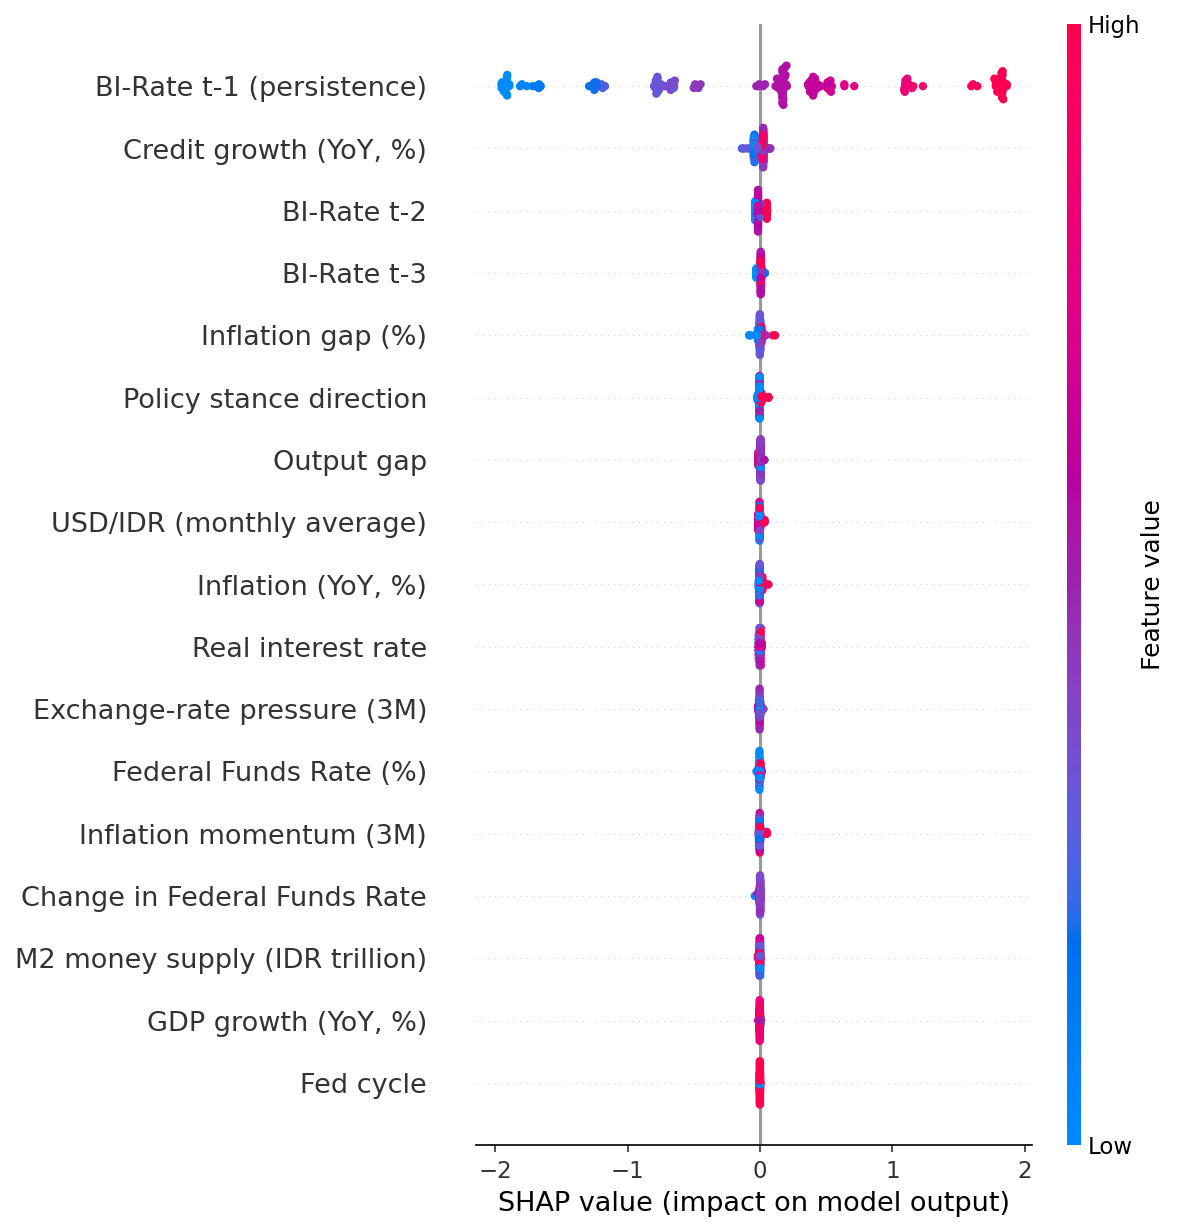
\includegraphics[width=\columnwidth]{fig_shap_summary.png}}
\caption{SHAP summary plot of the Random Forest model. The one-month lag dominates; macroeconomic contributors follow at an order of magnitude below.}
\label{fig:shap}
\end{figure}

\begin{figure*}[htbp]
\centerline{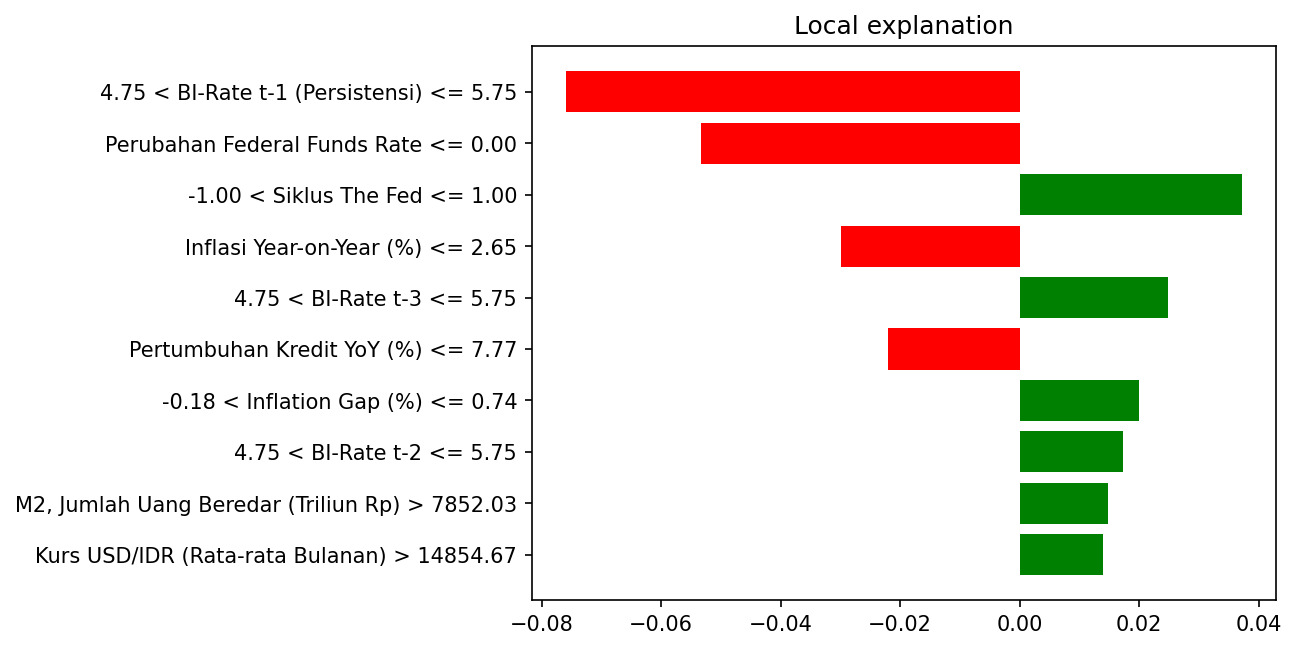
\includegraphics[width=0.62\textwidth]{fig_lime_explanation.png}}
\caption{LIME local explanation for the July 2025 control month on the Random Forest. Bars give each binned condition's contribution: red pushes the prediction down, green pushes it up. BI-Rate persistence leads, but the change in the Federal Funds Rate (\textit{Perubahan Federal Funds Rate}) ranks second and credit growth (\textit{Pertumbuhan Kredit YoY}) only sixth, against SHAP's ordering in Table~\ref{tab:shap}. The surrogate $R^2$ for this month is 0.0022.}
\label{fig:lime}
\end{figure*}

\subsection{Narratives and Expert Validation}
For each explained month, GPT-4o produces a structured narrative: a numeric summary, factors pushing the prediction up, factors holding it down, a recap of dominant factors, and an expert-judgment disclaimer. The following excerpt is the Random Forest narrative for July 2025, abridged and translated from the Indonesian original the system produces for its intended audience.

\begin{quote}\small\itshape
The BI-Rate prediction for July 2025 is 5.25\%. [\ldots] One factor pushing the prediction higher is the real interest rate, at 3.13\% against 3.63\% the previous month, shifting the prediction by about 4\% of this month's total influence. [\ldots] The most dominant factor holding the prediction lower is the previous month's BI-Rate, stable at 5.50\%. This reflects Bank Indonesia's practice of maintaining rate continuity and carries about 73\% of the total influence. Credit growth also holds the prediction lower, with about 15\%, having fallen from 7.57\% to 6.67\%. [\ldots] This explanation rests on patterns the model learned from historical data, so deeper economic interpretation still requires expert analysis.
\end{quote}

Every quantity there is checkable. The 73\% is the one-month lag alone (local SHAP $-0.5946$ of 0.8145 total absolute contribution); the 75.5\% in Section~\ref{sec:xai} is larger because it groups all three BI-Rate lags. Credit growth's 15\% corresponds to $-0.1238$, the real interest rate's 4\% to $+0.0319$. Nothing appears that is absent from the SHAP output, and no causal claim is made beyond the direction of the shift.

The Bank Indonesia expert scored the system 3.99 of 5 overall across 96 items. Per-model means were LSTM 4.21, BiLSTM 4.00, Random Forest 3.92, and XGBoost 3.83---notably, the expert ranking does not follow the accuracy ranking: the most accurate model (Random Forest) produces persistence-dominated explanations that the expert found less economically rich, showing that accuracy and explanation quality are distinct dimensions.

The two extremes of the feature-importance item are independently corroborated by ablation. LSTM, which scored full marks on that item for July 2025, is the model whose SHAP attributions ablation confirms: SHAP ranks the output gap and the Federal Funds Rate among its top drivers, and those are precisely the features whose removal hurts LSTM most (RMSE 0.1620$\rightarrow$0.2805 and $\rightarrow$0.1963). XGBoost, which scored lowest on that item, is the model whose attributions ablation contradicts: SHAP ranks credit growth first with a 45--54\% share, yet removing credit growth \emph{improves} XGBoost RMSE from 0.2207 to 0.2038. An apparently subjective expert judgment thus traces back to standalone quantitative evidence. The items ``absence of hallucination'' and ``narrative consistency with displayed SHAP values'' received full marks (5/5) in all assessments, while lay readability scored 3, indicating the main improvement direction.

\subsection{Limitations}
Five limitations qualify these results: (1) expert validation involved a single (albeit highly qualified) rater, so no inter-rater statistics are possible; (2) only nine change months exist in the test window, making directional rates sensitive to individual months; (3) during screening, imputation preceded splitting, though the canonical winner (forward fill) is causal and the affected alternatives did not win; (4) a regularization probe (LSTM with L2 = 0.01) reaches test RMSE 0.119 and beats the canonical Random Forest in all 120 three-seed ensembles it forms, but it sits outside the locked registry and awaits confirmation as a tuned configuration; and (5) the narrative layer calls a proprietary API, so a central-bank deployment should host the LLM locally, noting that only aggregated SHAP values are transmitted.

\section{Conclusion and Future Work}
We presented an end-to-end system that predicts Indonesia's BI-Rate from 12 macroeconomic indicators and explains each prediction through exact SHAP attribution, LIME direction checks, and strictly grounded LLM narratives. Two claims survive the evaluation. First, aggregate accuracy is the wrong measure on this series: it is largely inherited from interest-rate smoothing, which the system itself quantifies (SHAP 0.9611 on the one-month lag), and a three-feature lag-only model beats the full configuration on it. Separating the nine rate-change months reverses the ranking---BiLSTM and LSTM reach 67\% directional accuracy there against Random Forest's 33\%---and leave-one-out ablation traces that capability to the macroeconomic block rather than to persistence. The models' predictive value is therefore real but narrow, concentrated in exactly the months that matter for policy analysis. Second, expert validation (3.99/5, zero hallucination findings) supports the transparency claim, and the expert's per-model judgments turn out to be reproducible from ablation evidence obtained independently of the questionnaire.

Future work includes multi-expert validation with inter-rater reliability, larger tuning budgets and DL ensembles on the existing pipeline, confirmation of the L2 regularization lead as a tuned configuration, explicit handling of the asymmetric response to tightening cycles that produces the one-sided misses, and extension of the methodology---which is transferable by design---to other policy rates and central banks.

\section*{Acknowledgment}
The authors thank the Bank Indonesia monetary economist who evaluated the system's explanation outputs.

\begin{thebibliography}{00}
\bibitem{taylor1993} J. B. Taylor, ``Discretion versus policy rules in practice,'' \emph{Carnegie-Rochester Conference Series on Public Policy}, vol. 39, pp. 195--214, 1993.
\bibitem{chakraborty2017} C. Chakraborty and A. Joseph, ``Machine learning at central banks,'' Bank of England Staff Working Paper No. 674, London, 2017.
\bibitem{lundberg2017} S. M. Lundberg and S.-I. Lee, ``A unified approach to interpreting model predictions,'' in \emph{Advances in Neural Information Processing Systems 30 (NeurIPS)}, 2017, pp. 4765--4774.
\bibitem{ribeiro2016} M. T. Ribeiro, S. Singh, and C. Guestrin, ``\,`Why should I trust you?': Explaining the predictions of any classifier,'' in \emph{Proc. 22nd ACM SIGKDD Int. Conf. Knowledge Discovery and Data Mining}, 2016, pp. 1135--1144.
\bibitem{clarida1999} R. Clarida, J. Gal\'{i}, and M. Gertler, ``The science of monetary policy: A new Keynesian perspective,'' \emph{Journal of Economic Literature}, vol. 37, no. 4, pp. 1661--1707, 1999.
\bibitem{bussmann2021} N. Bussmann, P. Giudici, D. Marinelli, and J. Papenbrock, ``Explainable machine learning in credit risk management,'' \emph{Computational Economics}, vol. 57, pp. 203--216, 2021.
\bibitem{calik2025} S. S. \c{C}al{\i}k, A. Aky\"{u}z, Z. H. Kilimci, and K. \c{C}olak, ``Explainable-AI powered stock price prediction using time series transformers: A case study on BIST100,'' arXiv preprint arXiv:2506.06345, 2025.
\bibitem{yu2023} X. Yu, Z. Chen, Y. Ling, et al., ``Temporal data meets LLM---Explainable financial time series forecasting,'' arXiv preprint arXiv:2306.11025, 2023.
\bibitem{breiman2001} L. Breiman, ``Random forests,'' \emph{Machine Learning}, vol. 45, no. 1, pp. 5--32, 2001.
\bibitem{chen2016} T. Chen and C. Guestrin, ``XGBoost: A scalable tree boosting system,'' in \emph{Proc. 22nd ACM SIGKDD Int. Conf. Knowledge Discovery and Data Mining}, 2016, pp. 785--794.
\bibitem{hochreiter1997} S. Hochreiter and J. Schmidhuber, ``Long short-term memory,'' \emph{Neural Computation}, vol. 9, no. 8, pp. 1735--1780, 1997.
\bibitem{schuster1997} M. Schuster and K. K. Paliwal, ``Bidirectional recurrent neural networks,'' \emph{IEEE Transactions on Signal Processing}, vol. 45, no. 11, pp. 2673--2681, 1997.
\bibitem{akiba2019} T. Akiba, S. Sano, T. Yanase, T. Ohta, and M. Koyama, ``Optuna: A next-generation hyperparameter optimization framework,'' in \emph{Proc. 25th ACM SIGKDD Int. Conf. Knowledge Discovery and Data Mining}, 2019, pp. 2623--2631.
\end{thebibliography}

\end{document}
